\documentclass[a4paper]{article}
\usepackage[utf8]{inputenc}
\usepackage{fullpage}
\usepackage{csquotes}
\usepackage[ngerman]{babel}
\usepackage{biblatex}
\usepackage{float}
\usepackage{graphicx}
\usepackage{subfigure}
\usepackage[format=plain,labelfont=bf,up]{caption}
\usepackage{hyperref}
\bibliography{documentation.bib}
\title{Impaired Vision \\ Ein Augmented-Reality-Simulator für Sehstörungen}
\author{Willi Schönborn}
\date{\today}
\begin{document}

\begin{figure}[H]
\centering

\includegraphics{beuth.png}
\maketitle
\end{figure}

\section*{Einleitung}
Als Teil der Lehrveranstaltung \textit{Multimediatechnik Vertiefung} an der \textit{Beuth Hochschule für Technik Berlin} soltel im Rahmen einer Semesterarbeit ein Projekt mit Bezügen zu den Bereichen Multimedia und Wahrnehmung entstehen. Das Ziel dieses Dokumentes ist es die Ideen, Konzepte sowie die Ergebnisse dieses Projektes vorzustellen.

\section*{Augmented Reality}
Unter \textit{Augmented Reality} versteht man die computergestützte Erweiterung der Realitätswahrnehmung \cite{WP-AR2011}. Es gibt diverse doch sehr ausschweifende Definitionen dieses Begriffs. Innerhalb dieses Dokumentes wird Augmented Reality als die visuelle Darstellung von Informationen verstanden, also die Ergänzung von Bildern oder Videos mit computergenerierten Zusatzinformationen oder virtuellen Objekten mittels Einblendung/Überlagerung \cite{WP-AR2011}. Abbildung \ref{augmented-reality} zeigt eine typische Anwendung der Prinzipien von Augmented Reality anhand einer Anwendung für Smartphones, die es erlaubt geographische Informationen über Objekte die sich im Sichtfeld des Betrachters befinden direkt über das Kamerabild zu legen. Mithilfe solcher Augmented-Reality-Anwendungen entsteht eine neuartige Wahrnehmung der Umgebung. Genau an dieser Stelle setzt die Idee dieses Projektes an: Eine ungewohnte Sicht auf gewohnte Dinge ermöglichen.

\begin{figure}[H]
\centering
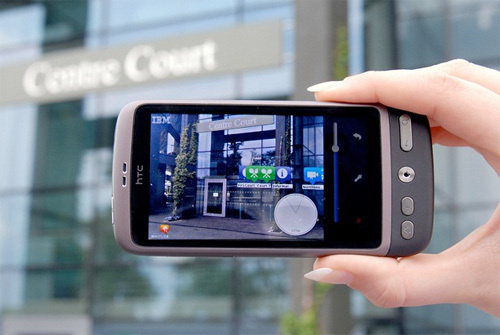
\includegraphics[width=0.9\textwidth, trim=0 40 0 50, clip=true]{augmented-reality.jpg}
\caption{Augmented Reality Anwendung}
\label{augmented-reality}
\end{figure}

\newpage

\section*{Idee}
Das Ergebnis dieses Projektes sollte ein Anwendung für Mobiltelefone werden, die es ermöglicht diverse Sehstörungen für normalsichtige Menschen zu simulieren. In der schriftlichen Projektidee wurden als mögliche Kandidaten für die Sehstörungen, die simuliert werden können Rot-Grün-Sehschwäche, Gelb-Blau-Sehschwäche sowie Kurzsichtigkeit aufgeführt. Nach einigen Recherchen sowie dem ausgiebigen Studium von \textit{Sensation and Perception} \cite{Goldstein2009} wurde relativ schnell deutlich, dass umgangssprachliche Vereinfachungen wie \textit{farbenblind} oder \textit{Rot-Grün-Schwäche} differenzierter betrachtet werden müssen um ein zufriedenstellendes Projektergebis zu erreichen. Zu diesem Zweck werden im nächsten Kapitel alle Sehstörungen näher behandelt und analysiert, die später simuliert werden sollen.

\section*{Sehstörungen}
Insgesamt wurden fünf unterschiedliche Sehschwächen ausgewählt wobei der Schwerpunkt klar auf den Farbfehlsichtigkeiten liegt. Neben der klassischen Myopie, der Kurzsichtigkeit, sowie den drei Vertretern der Dichromasie, der teilweisen Farbblindheit \cite{WP-D2011} wird auch die Achromasie, die komplette Farbenblindheit, behandelt. 

\subsection*{Myopie}

\begin{figure}[H]
\centering
\subfigure[Normalsichtigkeit]{
    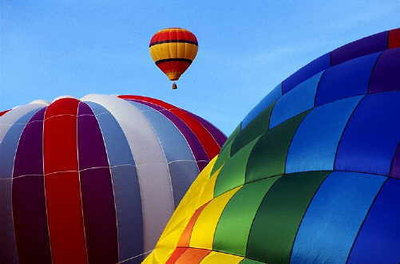
\includegraphics[width=0.475\textwidth]{balloons.jpg}
}
\subfigure[Myopie (Kurzsichtigkeit)]{
    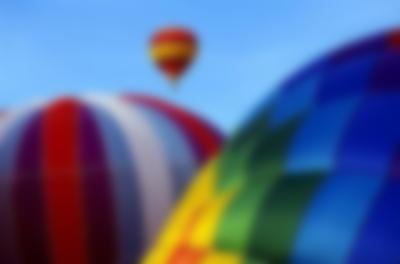
\includegraphics[width=0.475\textwidth]{balloons-myopia.jpg}
}
\caption{Myopie im Vergleich}
\end{figure}

\subsection*{Protanopie}

\begin{figure}[H]
\centering
\subfigure[Normalsichtigkeit]{
    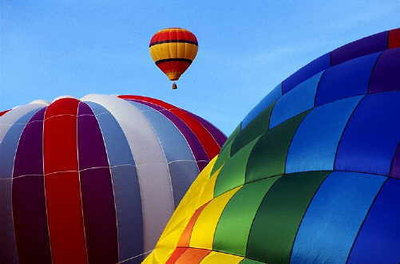
\includegraphics[width=0.475\textwidth]{balloons.jpg}
}
\subfigure[Protanopie]{
    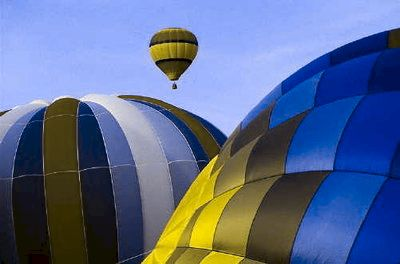
\includegraphics[width=0.475\textwidth]{balloons-protanope.jpg}
}
\caption{Protanopie im Vergleich}
\end{figure}

\subsection*{Deuteranopie}

\begin{figure}[H]
\centering
\subfigure[Normalsichtigkeit]{
    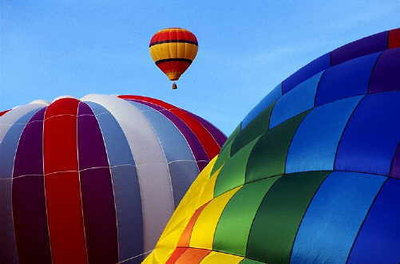
\includegraphics[width=0.475\textwidth]{balloons.jpg}
}
\subfigure[Deuteranopie]{
    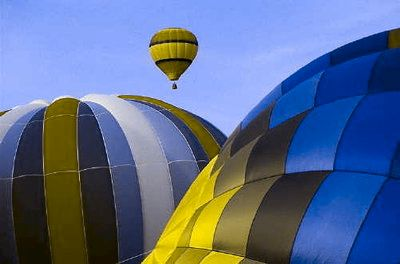
\includegraphics[width=0.475\textwidth]{balloons-deuteranope.jpg}
}
\caption{Deuteranopie im Vergleich}
\end{figure}

\subsection*{Tritanopie}

\begin{figure}[H]
\centering
\subfigure[Normalsichtigkeit]{
    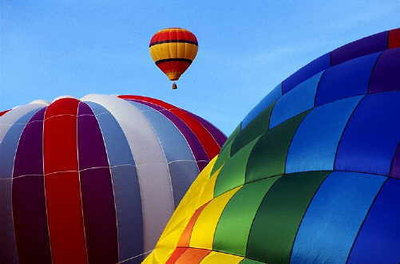
\includegraphics[width=0.475\textwidth]{balloons.jpg}
}
\subfigure[Tritanopie]{
    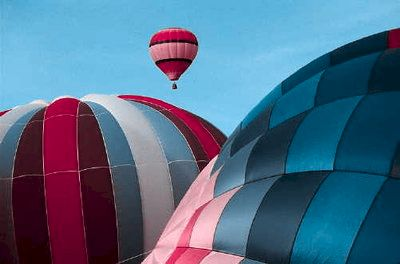
\includegraphics[width=0.475\textwidth]{balloons-tritanope.jpg}
}
\caption{Tritanopie im Vergleich}
\end{figure}

\subsection*{Achromasie}

\begin{figure}[H]
\centering
\subfigure[Normalsichtigkeit]{
    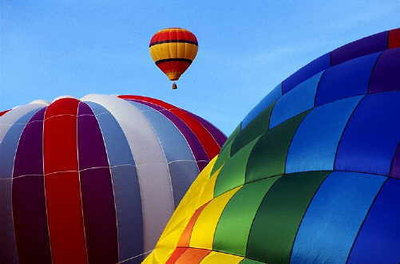
\includegraphics[width=0.475\textwidth]{balloons.jpg}
}
\subfigure[Achromasie]{
    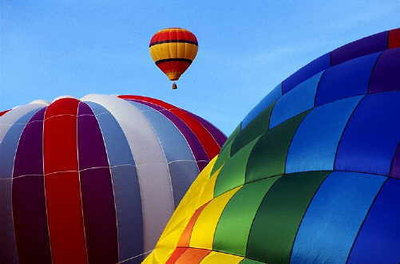
\includegraphics[width=0.475\textwidth]{balloons-achromate.jpg}
}
\caption{Achromasie im Vergleich}
\end{figure}

\newpage

\nocite{ANDROID}
\nocite{GIZMODO}
\nocite{VISCHECK}
\nocite{IBFB}
\printbibliography

\listoffigures

\end{document}

